\documentclass[UTF8]{ctexart}
%\usepackage{fontspec}
\usepackage{float}
\usepackage{booktabs}
\usepackage{verbatim}
\usepackage{amsthm}
\usepackage{algorithm}
\usepackage{threeparttable,booktabs}
\usepackage[noend]{algpseudocode}
\usepackage{indentfirst,amssymb,amsmath,color,graphicx,pifont,amsmath}


\numberwithin{equation}{section}
\graphicspath{{./pic/}}
\usepackage[T1]{fontenc}

%% 采取A4纸张,页边距采取(上下2.54cm,左右3.17cm,页眉1.5cm,页脚1.75cm)
%% 设置1.5倍行间距. 注意, word和latex中多倍行距的默认系数是不一样的, 前者是1.3, 后者是1.2. 想要在Latex中实现Word中的"1.5"倍行距,实际倍数为1.5*1.3/1.2=1.625
%% (但是本人更喜欢1.5倍, 故保留)
\usepackage{geometry}
\geometry{a4paper,left=3.18cm,right=3.18cm,top=2.54cm,bottom=2.54cm,headheight=1.5cm,footskip=1.75cm }
\renewcommand\baselinestretch{1.5}

\usepackage{fancyhdr}  
\usepackage{lastpage}
\fancyhf{} 


%% "目录"二字用三号字、黑体、居中书写,“目”与“录”之间空一格。内容用小四号字、宋体。
%% 目录里包括正文层次的标题序号、参考文献、致谢、附录等标题和页码。
\renewcommand{\contentsname}{ \heiti\zihao{3}目\ 录}
%\usepackage{tocloft}
%\renewcommand{\cftsecfont}{\zihao{-4}} 
%\renewcommand{\cftsubsecfont}{\zihao{-4}}

%% 一级标题采用三号字黑体居中,上下各空一行;
%% 二级及以下标题用小四号字黑体;
\ctexset{
  section = {
    format = \zihao{3}\centering\bfseries\heiti, 
    name = {第,章},
    number = \arabic{section},
    aftername = \quad,  
	beforeskip = 1.0\baselineskip,  
    afterskip = 1.0\baselineskip,   
  },
  subsection = {format = \zihao{-4}\heiti, },
  subsubsection = {format = \zihao{-4}\heiti, }
}


\newtheorem{theorem}{\color{black}\indent{定理}}[section]
\newtheorem{lemma}{\color{black}\indent{引理}}[section]
\newtheorem{proposition}{\color{black}\indent{命题}}[section]
\newtheorem{definition}{\color{black}\indent{定义}}[section]
\newtheorem{remark}{\color{black}\indent{注}}[section]
\newtheorem{corollary}{\color{black}\indent{推论}}[section]
\newtheorem{example}{\color{black}\indent{例}}[section]
%\newtheorem{proof}{\color{black}\indent{证明}}
\newtheorem{solution}{\color{black}\indent{解}}
\newcommand{\bt}[2]{\begin{center}{\bf\heiti\S {#1}\hbox{#2}}\end{center}}
\newcommand{\wx}[1]{$^{[#1]}$}
\newcommand{\w} [1]{\re {[#1]}}
\newtheorem{fig}[figure]{\it figure}


%% 图、表、公式等与正文之间要有一行的间距;文中的图,表,附注,公式采用阿拉伯数字
%% 分章(或连续)编号。如:图 2-5,表 3-2,公式(5-1)等。若图或表中有附注,采用英文小写字母顺序编号
\usepackage{graphicx}
\usepackage{subfigure} 
%subfigure与tocloft同时使用会出错, 请注意
%\usepackage{pstricks,pst-plot,pst-func}
%\usepackage{pspicture}
%\usepackage{curves}


\allowdisplaybreaks
%\include{rgb}

%% For creating math operators
\DeclareMathOperator*{\argmax}{argmax}
\def\d{{\mathrm d}}

\def\A{{\mathcal{A}}}
\def\H{{\mathcal{H}}}
\def\G{{\mathcal G}}
\def\F{{\mathcal F}}
\def\U{{\mathcal U}}
\def\V{{\mathcal V}}

\def\eps{\varepsilon}
\def\ds{\displaystyle}

\def\<{{\langle }}
\def\>{{\rangle }}

\floatname{algorithm}{算法}


\begin{document}

%% 封面本体
%%\title{ 在时间并行算法中学习粗网格传播器}
%%\author
%%{\hspace{1cm}           \\
%\zihao{-4}\scriptsize{吉林大学数学学院\quad 信息与计算科学%\quad 长春~130012}                         \\
%}                        
%\date{}


%% 毕业论文封皮要求选用 120 克白色封面纸打印输出
%% 标题用二号字、黑体、加粗; 姓名等用四号字、宋体、加粗
\begin{titlepage}
    \centering
    \vspace{0cm}
    \makebox[\textwidth][c]{%
        
\includegraphics[width=1.2\textwidth]{JLU} 
    }

    \vspace{3cm}
    {
    \renewcommand{\arraystretch}{1.8}  
    \begin{tabular}{rl}
        \zihao{3} \textbf{中文题目}
        &\underline{\makebox[10cm]{\huge\bfseries\heiti 在时间并行算法中学习粗网格}}  \\
        &\underline{\makebox[10cm]{\huge\bfseries\heiti 传播器}}  \\
    \end{tabular}
    }

    \vspace{5.5cm}
    {\zihao{4}\bfseries
    \renewcommand{\arraystretch}{1.2}  
    \begin{tabular}{llll}
        \textbf{学生姓名:} & \underline{\makebox[4cm]{小明}} & \textbf{专业:} & \underline{\makebox[4cm]{计算机科学技术}} \\
        \textbf{层次年级:} & \underline{\makebox[4cm]{2020本科}} & \textbf{学号:} & \underline{\makebox[4cm]{2111110101101}} \\
        \textbf{指导教师:} & \underline{\makebox[4cm]{}} & \textbf{职称:} & \underline{\makebox[4cm]{教授}} \\
        \textbf{学习中心:} & \underline{\makebox[4cm]{长春}} & \textbf{成绩:} & \underline{\makebox[4cm]{}} \\
    \end{tabular}
    }

    \vspace{2.5cm}

    {\rightline{\bfseries\zihao{-2}2024年3月14日}}

\end{titlepage}


\thispagestyle{empty}


\newpage
%% 页眉从摘要开始,本科生设为“吉林大学网络教育xx届本科生毕业设计(论文)”,采用宋体五号字居中书写
%% 页码放在页脚中(第 X 页 共 X 页)(宋体小五号),从正文开始,居中书写
\pagestyle{fancy} 
\chead{\zihao{5} \textbf{吉林大学网络教育}2020届本科生毕业设计(论文)}
\cfoot{}

%% 摘要本体
\vspace*{-8mm}
%% “摘要”二字中间空两格、小二号字、黑体、居中
\begin{center}
	\zihao{-2} {\heiti{摘\ \ \ 要:}}
\end{center}
\renewcommand\baselinestretch{1.5} 

%% 摘要内容用四号字、宋体, “关键词”三字加粗,各关键词之间要有空格
{\zihao{4}时间并行算法中的一个重要类别是Parareal算法, 它广泛应用于解决演化方程. 为了实现有效的加速, 算法中选择合适的粗网格传播器至关重要. 在这项工作中, 我们探讨了学习型粗网格传播器的使用. 基于误差估计框架, 我们提出了一种构建具有稳定性和相容精度的粗网格传播器的方法. 此外, 我们为所得Parareal算法提供了初步的数学保证. 在各种设置上的数值实验, 例如线性扩散模型、Allen-Cahn模型和粘性Burgers模型, 表明与一些传统且广泛使用的粗网格传播器相比, 学习型粗网格传播器可以显著提高并行效率. 

\vskip5mm

%% “关键词”三字加粗,各关键词之间要有空格
{\textbf{关键词:}} 椭圆问题; 单步法; 收敛方法; 机器学习}


\newpage 

\begin{center}
\tableofcontents
\end{center}

\newpage
\addtocounter{page}{1}
\cfoot{\zihao{-5}第 \thepage 页\ 共 \pageref{LastPage} 页}

%% 正文本体
%% 一级标题采用三号字黑体居中,上下各空一行;二级及以下标题用小四号字黑体;正文用小四号字宋体。
\section{绪论}
\subsection{研究背景和问题模型}
本文致力于使用机器学习技术加速一类针对抛物问题的Parareal求解器. 设定一个固定的终止时间 \( T > 0 \). 考虑以下初始值问题, 对于 \( u \in C((0,T];D(\A))\cap C([0,T];\H) \):
\begin{equation}\label{eqn:pde}
	\left \{
	\begin{aligned}
		&u' (t) + \A u(t) = f(t), \quad 0<t<T,\\
		& u(0)=u^0 ,
	\end{aligned}\right .
\end{equation}
其中 \( u^0 \in \H \) 是初始数据, \( f : [0,T] \to \H \) 是给定的强制项, 而 \( \A \) 是一个正定的、自伴的、线性算子, 拥有紧逆的算子, 定义在带有内积 \( (\cdot , \cdot ) \) 的希尔伯特空间 \( \H \) 上(带有诱导范数 \( \|\cdot\| \)), 其定义域 \( D(\A) \) 在 \( \H \) 中稠密. 这个模型在实际应用中有非常广泛的应用, 其有效的数值模拟具有极大的重要性, 并受到了大量关注 (\cite{thomee2007galerkin}). 

模型 \eqref{eqn:pde} 的数值解通常采用时间离散化, 提出了各种时间步进格式;具体内容参见专著 \cite{thomee2007galerkin}. 这些格式通常逐步进行, 过程本质上是顺序的. 这是模型 \eqref{eqn:pde} 数值解的主要瓶颈, 尤其是在大时间尺度上. 在开创性的工作 \cite{LionsMadayTurinici:2001} 中, Lions、Maday 和 Turinici 提出了一种称为Parareal算法的方法, 用于以时间并行的方式求解演化模型. 该方法已成为在分布式计算在空间上饱和时利用高度并行系统的基础工具. 自从它的诞生以来, 这类方法已成功应用于众多不同的实际应用, 例如期权定价 \cite{BalMaday:2002,PagesPironneau:2016}、多尺度动力学 \cite{ArielKim:2016,Engblom:2009}、随机PDE \cite{BrehierWang:2020} 和分数扩散 \cite{LiHu:2021,XuHesthaven:2015}. 

Parareal算法基于两个求解器, 一个是粗网格传播器(coarse propagator, CP), 精度低但足够快以便顺序应用, 另一个是精度高的细网格传播器(fine propagator, FP), 在时间上并行应用. 在每次迭代中, CP在每个子域上顺序运行, 然后FP作为修正并行运行. 有关CP和FP如何交互的详细信息, 请参阅第 \ref{ssec:Parareal} 节. CP通常基于标准数值求解器的一步或几步, 实际上, 它通常是使用较低分辨率的数值积分器, 例如更大的时间步长大小, 以有效地向前传播信息. 理想情况下, Parareal算法可以以CP的效率达到FP的精度. 在现代多核计算机架构上实现所需的加速, CP的选择至关重要. 尽管如此, CP的最佳选择仍然极为非平凡. 更糟糕的是, 对于带有非平滑数据的模型 \eqref{eqn:pde}, 使用标准向后欧拉CP的Parareal算法的收敛性在某种程度上受限 \cite{FriedhoffSouthworth:2021,Mathew:2010,Wu:IMA2015,yang2021robust}, 这本质上限制了可实现的效率, 参见下面 \eqref{eqn:conv-1} 的精确陈述. 这个问题也出现在其他常用的CP上 \cite[表 1 和 2]{FriedhoffSouthworth:2021}. 这些观察自然引出了一个有趣的问题:是否可以通过适当修改CP来提高Parareal算法的收敛速度. 



\subsection{本文贡献和文章架构}
在这项工作中, 我们提出了一个创新且易于实现的框架, 用于设计针对问题 \eqref{eqn:pde} 的Parareal算法中的CP. 它基于误差估计框架, 并遵循使用学习来解决科学计算挑战的普遍范式(\cite{FriedhoffSouthworth:2021,GanderVandewalle:2007,Southworth:2019,yang2021robust}). 具体来说, 基于在误差估计框架中推导出的分析收敛因子, 我们构造了一个学习型粗网格传播器(learned coarse propagator, LCP), 以最小化收敛因子的上界. 这样, LCP就是针对FP特别学习的, 这与常规选择中CP几乎对FP的选择无知大相径庭. 我们提供了一种构建拥有理想特性(例如稳定性和准确性)的CP的方法. 我们对该框架进行了初步分析, 表明LCP确实可以实现线性演化问题的预期目标. 我们展示了几个线性和非线性问题的数值实验, 包括线性扩散模型、Allen-Cahn模型和粘性Burgers方程, 以说明这种方法的优越性. 数值结果表明, 与使用后向欧拉格式(或其他流行的单步方法)作为CP的传统选择相比, 使用学习技术始终能够提高性能. 


这项工作大体上, 遵循了用于科学计算的学习数值算法的普遍范式, 它结合了数学驱动的、手工设计的一般算法结构与针对特定任务类别的数据驱动适应(\cite{Bar-Sina:2019,GreenfeldKimmel:2019,GuoLi:2022,HuangLiXi:2023,IbrahimRuprecht:2023,Mishra:2019}). 例如, Guo等人提出了一种机器学习方法, 它能够自动学习求解常微分方程初值问题的有效解算器, 基于Runge-Kutta积分器, 并学习针对特定族群的微分方程的高阶积分器(\cite{GuoLi:2022}). LCP在设计新的并行算法中的应用也得到了探索 (\cite{AgbohDogar:2020,IbrahimRuprecht:2023,NguyenTsai:2023,YallaEngquist:2018}). Yalla和Engquist 探索了使用神经网络近似高维谐振子和局部多尺度问题的相位图作为CP(\cite{YallaEngquist:2018}). Agboh等人使用前馈深度神经网络作为CP来积分ODE, 并观察到性能的提升(\cite{AgbohDogar:2020}). Nguyen和Tsai 使用监督学习来提高波传播的效率(\cite{NguyenTsai:2023}). Ibrahim等人提出使用物理信息神经网络(PINN)作为CP, 并展示了其在Black-Scholes方程上相比数值CP的加速性能(\cite{IbrahimRuprecht:2023}). 本文继续沿着这一活跃的研究路线探索使用学习概念增强并行算法(\cite{AgbohDogar:2020,IbrahimRuprecht:2023,NguyenTsai:2023,YallaEngquist:2018}). 但与众不同的是, 它显式地将分析洞察融入学习过程中, 即稳定性和相容性, 因此本文提出的LCP具有严格的数学保证(\cite{jin2023learning}). 更具体地说,我们的工作可以概括为:
\begin{itemize}
	\item[(i)]  设计算法学习Parareal 算法中的学习型粗网格传播器. 
	\item[(ii)]  提供理论保证, 学习型粗网格传播器关于网格比是鲁棒的. 
	\item[(iii)] 在三种抛物问题中的数值案例中, 说明学习型粗网格传播器大大加速了并行效率. 
\end{itemize}


\section{单步方法和并行算法}\label{sec:prelim}
首先, 我们描述了用于解决问题 \eqref{eqn:pde}的单步法的抽象框架, 并简要概述了并行算法. 对于这些主题的深入处理, 我们建议感兴趣的读者参考专著\cite{thomee2007galerkin}和综述\cite{gander201550}. 

\subsection{抛物方程的单步求解器}\label{ssec:single step}
为了在时间上离散化问题 \eqref{eqn:pde}, 我们将时间区间$(0,T)$分为$N$个等距子区间, 每个子区间长度为${\Delta t} = T/N$, 并设格点为$t_n = n{\Delta t}$, 其中$n=0,1,\ldots,N$. 然后, 单步求解器通过
\begin{equation}\label{eqn:semi}
	u^{n+1} = r({\Delta t} \A) u^{n} + {\Delta t} \sum_{i=1}^m p_i({\Delta t} \A)
	f(t_n+c_i\Delta t) ,\quad \text{对于}~0\le n\le N-1. 
\end{equation}
来近似解$u(t_{n+1})$. 
这里$r(\cdot)$和序列$\{p_i(\cdot)\}^m_{i=1}$是有理函数, ${c_i}$是$[0,1]$中的不同实数. 
下面我们对格式 \eqref{eqn:semi}提出以下条件:
\begin{itemize}
	\item[{\bf (P1):}] $| r (\lambda)|< 1$ 和 $|p_i(\lambda)|\le c$, 对所有$i=1,\ldots,m$, 对于任何${\Delta t}$和任何$\lambda > 0$都成立. 进一步, $p_i$的分子次数严格低于分母. 
	\item[{\bf (P2):}] 格式\eqref{eqn:semi}精确到$q$阶, 即
	$$  r (\lambda) = e^{-\lambda} + \mathcal{O}(\lambda^{q+1}),\quad \text{当}~\lambda\rightarrow0.$$
	\noindent 另外, 对于每个$0\le j\le q$, 
	$$ \sum_{i=1}^m c_i^j p_i(\lambda) - \frac{j!}{(-\lambda)^{j+1}}\Big(e^{-\lambda}
	- \sum_{\ell=0}^j \frac{(-\lambda)^\ell}{\ell!}\Big) = \mathcal{O}(\lambda^{q-j}),\quad \text{当}~\lambda\rightarrow0.$$
	\item[{\bf (P3):}] 有理函数$r(\lambda)$是强稳定的, 即$|r(\infty)|<1$. 
\end{itemize}

例如, 可以参考专著\cite[p.131]{thomee2007galerkin}了解满足条件{\bf{(P1)}}-{\bf{(P3)}}的有理函数的构造. {\bf{(P3)}}对于确保并行迭代的收敛性至关重要, 特别是对于非光滑问题数据(例如, $u^0\in\mathcal{H}$). 当$|r(\infty)| = 1$(例如, Crank-Nicolson和隐式Runge-Kutta的Gauss类型), 并行方法的收敛性取决于两个因素. 首先, $\A$的特征值必须有上界, 这通常不是抛物方程的情况. 其次, 粗步长和细步长之间的比率必须足够大, 具体值由$\A$的特征值的上界决定. 不满足(\textbf{P3})的格式可能会失去最优收敛率\cite[第8章]{thomee2007galerkin}. 

在实践中, 通常希望选择与$r (\lambda)$有相同分母的$p_i(\lambda)$, 即对于多项式$a_i(\lambda)$和$g(\lambda)$, 有
\begin{equation*}
	r (\lambda) = \frac{a_0(\lambda)}{g(\lambda)}\quad \text{和} \quad p_i(\lambda) = \frac{a_i(\lambda)}{g(\lambda)}, \quad \text{对于}~i=1,2,\ldots,m.
\end{equation*}
然后格式\eqref{eqn:semi}可以写成
\begin{equation*}
	g({\Delta t} \A) u^{n+1} = a_0({\Delta t} \A) u^{n} + {\Delta t} \sum_{i=1}^m a_i({\Delta t} \A) f(t_n+c_i\Delta t) ,\quad 1 \le n\le N-1.
\end{equation*}

以下误差估计适用于格式 \eqref{eqn:semi} (\cite[定理7.2和8.1]{thomee2007galerkin}). 
\begin{lemma}\label{lem:conv-00}
	假设条件{\bf{(P1)}}--{\bf{(P3)}}得到满足, 
	$u(t)$是问题\eqref{eqn:pde}的解, $u^n$
	是格式\eqref{eqn:semi}的解. 那么有
	\begin{equation*}%\label{eqn:semi-error}
		\|u^n - u(t_n)\|\leq
		c\, (\Delta t)^q \Big( t_n^{-q} \| u^0 \|
		+ t_n \sum_{\ell=0}^{q-1} \sup_{s\le t_n} \| \A^{q-\ell}f^{(\ell)}(s)  \| + \int_0^{t_n}
		\| f^{(q)}(s) \|\,\d s\Big),
	\end{equation*}
	如果$u_0\in \H$, $f^{(\ell)}\in C([0,T];\mathrm{Dom}(\A^{q-\ell})$对于$0\le \ell\le q-1$, 并且$f^{(q)} \in L^1(0,T; \H)$, 这里$Dom(\A)$代表$\A$的定义域.
\end{lemma}\medskip

 \begin{remark}\label{rem:conv-00}
	根据引理 \ref{lem:conv-00}, 在条件{\bf{(P1)}}-{\bf{(P3)}}下, 如果$f$和$u_0$满足某些兼容条件, 格式\eqref{eqn:semi}的解$u^n$会以$\mathcal{O}((\Delta t)^q)$的阶数收敛到精确解$u(t_n)$. 例如, 当\(\A = -\Delta\)时, 配备零狄利克雷边界条件, 要求是\( (-\Delta)^{\ell} f^{(q-\ell)} = 0 \) 在 \(\partial\Omega\) 对于 \(0 \le \ell \le q\). 为了规避这些严格条件, 假设格式\eqref{eqn:semi}严格精确到$q$阶, 即
	\[
	\sum_{i=1}^m c_i^j p_i(\lambda) - \frac{j!}{(-\lambda)^{j+1}}\Big( r (\lambda)
	- \sum_{\ell=0}^j \frac{(-\lambda)^\ell}{\ell!}\Big) = 0, \quad ~0\le j\le q-1.
	\]
	如果截断误差对于所有$f$和$u_0$都为零, 使得解是$t$中至多$p_0-1$阶的多项式, 则格式严格精确到$p_0 < p$阶. 
	虽然具有给定$m \in \mathbb{N}$的单步方法可能精确到$2m$阶(例如, Gauss--Legendre方法, \cite[第2.2节]{ehle1969pade}), 但它只能严格精确到最高\(m+1\)阶 \cite[引理5]{brenner1982single}. 
\end{remark}\medskip

\begin{remark}\label{rem:conv-01}
	如果积分器表现出L-稳定性, 即$r(\infty) = 0$, 则可以改进引理 \ref{lem:conv-00} 中的误差估计 (\cite[定理7.2]{thomee2007galerkin}). 
\end{remark}

\subsection{并行算法}\label{ssec:Parareal}
现在, 我们介绍单步积分器 \eqref{eqn:semi}的并行算法. 设$\Delta T = J \Delta t$为粗步长, $N_c = T/\Delta T\in \mathbb{N}$, 并表示$T_n = n\Delta T$. 数值传播器$\G$和$\F$分别对应粗和细时间网格. 通常, $\G$是一种便宜的、低阶数值方法(例如, 后向欧拉格式), 而$\F$由单步积分器 \eqref{eqn:semi}定义. 对于任何给定的初始数据$v\in \H$和$f\in C([0,T];\H)$, 粗和细网格传播器分别定义为
\begin{align}
	\G(T_n,\Delta T,v,f) &= R({\Delta T} \A) v + {\Delta T} \sum_{i=1}^{M} P_i({\Delta T} \A) f(T_n+C_i\Delta T) , \label{eqn:coarse-integrator}\\
	\F(t_n,\Delta t,v,f) &= r({\Delta t} \A) v + {\Delta t} \sum_{i=1}^{m} p_i({\Delta t} \A) f(t_n+c_i\Delta t). \label{eq: integrator}
\end{align}
其中, $M$和$m$分别表示粗网格传播器$\mathcal{G}$和细网格传播器$\mathcal{F}$的阶数, 以及$R$和$P$是粗网格传播器$\mathcal{G}$的有理函数, $r$和$p$是细网格传播器$\mathcal{F}$的. 并行迭代在下面的算法中给出. 

\begin{algorithm}[ht]

	\caption{并行算法. }
	\begin{algorithmic}[1]\label{alg:para}
		\State \textbf{初始化}:
		计算
		$U_0^{n+1} = \G(T_n,\Delta T, U_0^{n}, f)$, 其中$U_0^0 =u^0$, $n =0,1,...,N_c - 1$;
		\For {$k=0,1,\ldots,K$}
		\State 在每个子区间$[T_n,T_{n+1}]$上, 依次计算$j=0,1,2,\dots,J-1$
		$$  \widetilde U^{n, j+1}_{k} = \F(T_n+j \Delta t, \Delta t, \widetilde U^{n, j}_{k},f), $$
		初始值为$ \widetilde U^{n, 0}_{k} = U_k^n$, 并设$\widetilde U^{n+1}_{k} =  \widetilde U^{n, J}_{k}$. \vskip5pt
		\State 执行顺序校正, 即找到$U_{k+1}^{n+1}$通过
		$$  U_{k+1}^{n+1} = \G(T_n, \Delta T, U_{k+1}^{n}, f)  + \widetilde U^{n+1}_{k} -   \G(T_n, \Delta T, U_{k}^{n}, f) $$
		其中$U_{k+1}^0 = u^0$, 对于$n =  0,1,...,N_c - 1$;\vskip5pt
		\State 检查停止准则. 
		\EndFor
	\end{algorithmic}
\end{algorithm}

并行算法的收敛性已经得到了广泛研究(参见例如 \cite{Bal:2005,BrehierWang:2020,FriedhoffSouthworth:2021,GanderVandewalle:2007,Mathew:2010,Wu:IMA2015,WuZhou:2015,yang2021robust}). 
最近, 针对线性演化方程, 杨、袁和周证明了使用后向欧拉格式作为CP时, 存在一个阈值 $J_*>0$, 独立于 $\Delta T$、$\Delta t$ 和 $\A$ , 即在条件 {\bf{(P1)}}-{\bf{(P3)}} 下, 如果 $J\ge J_*$, 那么以下界限成立, 其中 $\gamma \approx 0.3$, 
\begin{equation}\label{eqn:conv-1}
	\max_{1 \le n\le N_c}\|  U_{k}^n - u^{nJ}  \| \le  c \,\gamma^k.
\end{equation}
这里, $U_k^n$ 表示并行解, $u^{nJ}$ 表示细时间步进解(\cite{yang2021robust}). 数值上观察到估计 \eqref{eqn:conv-1} 是精确的. 使用其他类型的CP时也会出现这个问题;文献 \cite{FriedhoffSouthworth:2021} 报告了当CP和FP都是两阶、单对角隐式Runge-Kutta格式(SDIRK-22)时, 最优的网格独立收敛因子 $\gamma \approx 0.26$, 而当两者都是SDIRK-33时, $\gamma \approx 0.15$, 对于 $J\in \{4, 8, 16, 32,64\}$. 这些观察自然地激发了以下问题:是否存在可以显著提高收敛性的CP, 同时在不同的$J$值上保持稳健性? 下面我们旨在学习新的CP来加速并行算法的收敛. 
% 此外, 数值上这些LCP对于非线性问题也表现出稳健性. 




我们在实验中取 $\nu \in \{1, 0.02 \}$.  对于 $\nu =1$, 我们检验了 $J=20$、$100$ 和 $\Delta t = 1/2000$(即 $\Delta T=1/100$ 和 $1/20$)的LCPs. 结果显示, 使用LCPs的Parareal算法的收敛速率约为 $0.04$, 对于更具挑战性的情况 $\nu =0.02$, 我们评估了 $J=10, 100$ 和 $\Delta t = 1/10000$(即 $\Delta T=1/1000$ 和 $1/100$)的LCPs. 对于 $J=10$, LCPs的收敛速率约为0.06, 而BE的收敛速率约为0.21. 值得注意的是, 对于 $J=100$ 在线性情况下, 比例 $\Delta T / \nu $ 保持不变, 因此它们的行为相似. 这一现象已经在 \cite{gander2020reynolds} 中对线性对流扩散案例进行了分析. 对于 $J=100$, LCPs 和BE 都表现出较慢的收敛. 



\section{总结}
我们探索了在Parareal算法中学习粗网格传播器的潜力, 以克服收敛阶数的障碍. 这种方法基于对线性演化问题的严格误差估计, 确保了LCPs具有高度理想的特性, 例如稳定性和相容性. 我们为CP的学习开发了一个系统化的方法. 数值实验完全证实了理论预测, 包括轻微非线性问题. 最值得注意的是, 即使对于高度非线性问题, LCPs仍然可以胜过经典的BE格式. 一个重要的问题是将这一思想扩展到更具挑战性的情况, 例如高度非线性问题、多尺度问题, 以及双曲问题 (\cite{DeSterck:2021,LiHu:2021}). 此外, 为其他并行时间算法(例如, 具有FCF平滑器的两级MGRIT算法 \cite{FriedhoffSouthworth:2021,Southworth:2019})开发学习策略也很有前景. 


\newpage
%% 参考文献要另起一页,一律放在正文后,不得放在各章之后. 参考文献作者最多写到第三位,余者写“等”。
%%(五号、黑体、顶格)格式:[1] 作者. 文题. 刊名,年,卷号(期号):起~止页码(仿宋体、五号)
 \setlength{\baselineskip}{14pt}
 \addcontentsline{toc}{section}{参考文献}
 \bibliographystyle{abbrv}
 \bibliography{refer}

\newpage
%% “致 谢”二字中间空一格、三号字、黑体、居中。
%% 内容限 1 页,采用小四号宋体。
\addcontentsline{toc}{section}{致谢}
\section*{致\ 谢}
在此,我要感谢我的导师和同事对我的支持和帮助。

\newpage

\appendix
\addcontentsline{toc}{section}{附录} 
\section*{附录}
\renewcommand{\thesubsection}{\Alph{subsection}}

\subsection{显式公式}\label{app:coarse}





在图 \ref{fig:app_2} 中 

\begin{figure} [tbhp!]
	\centering
	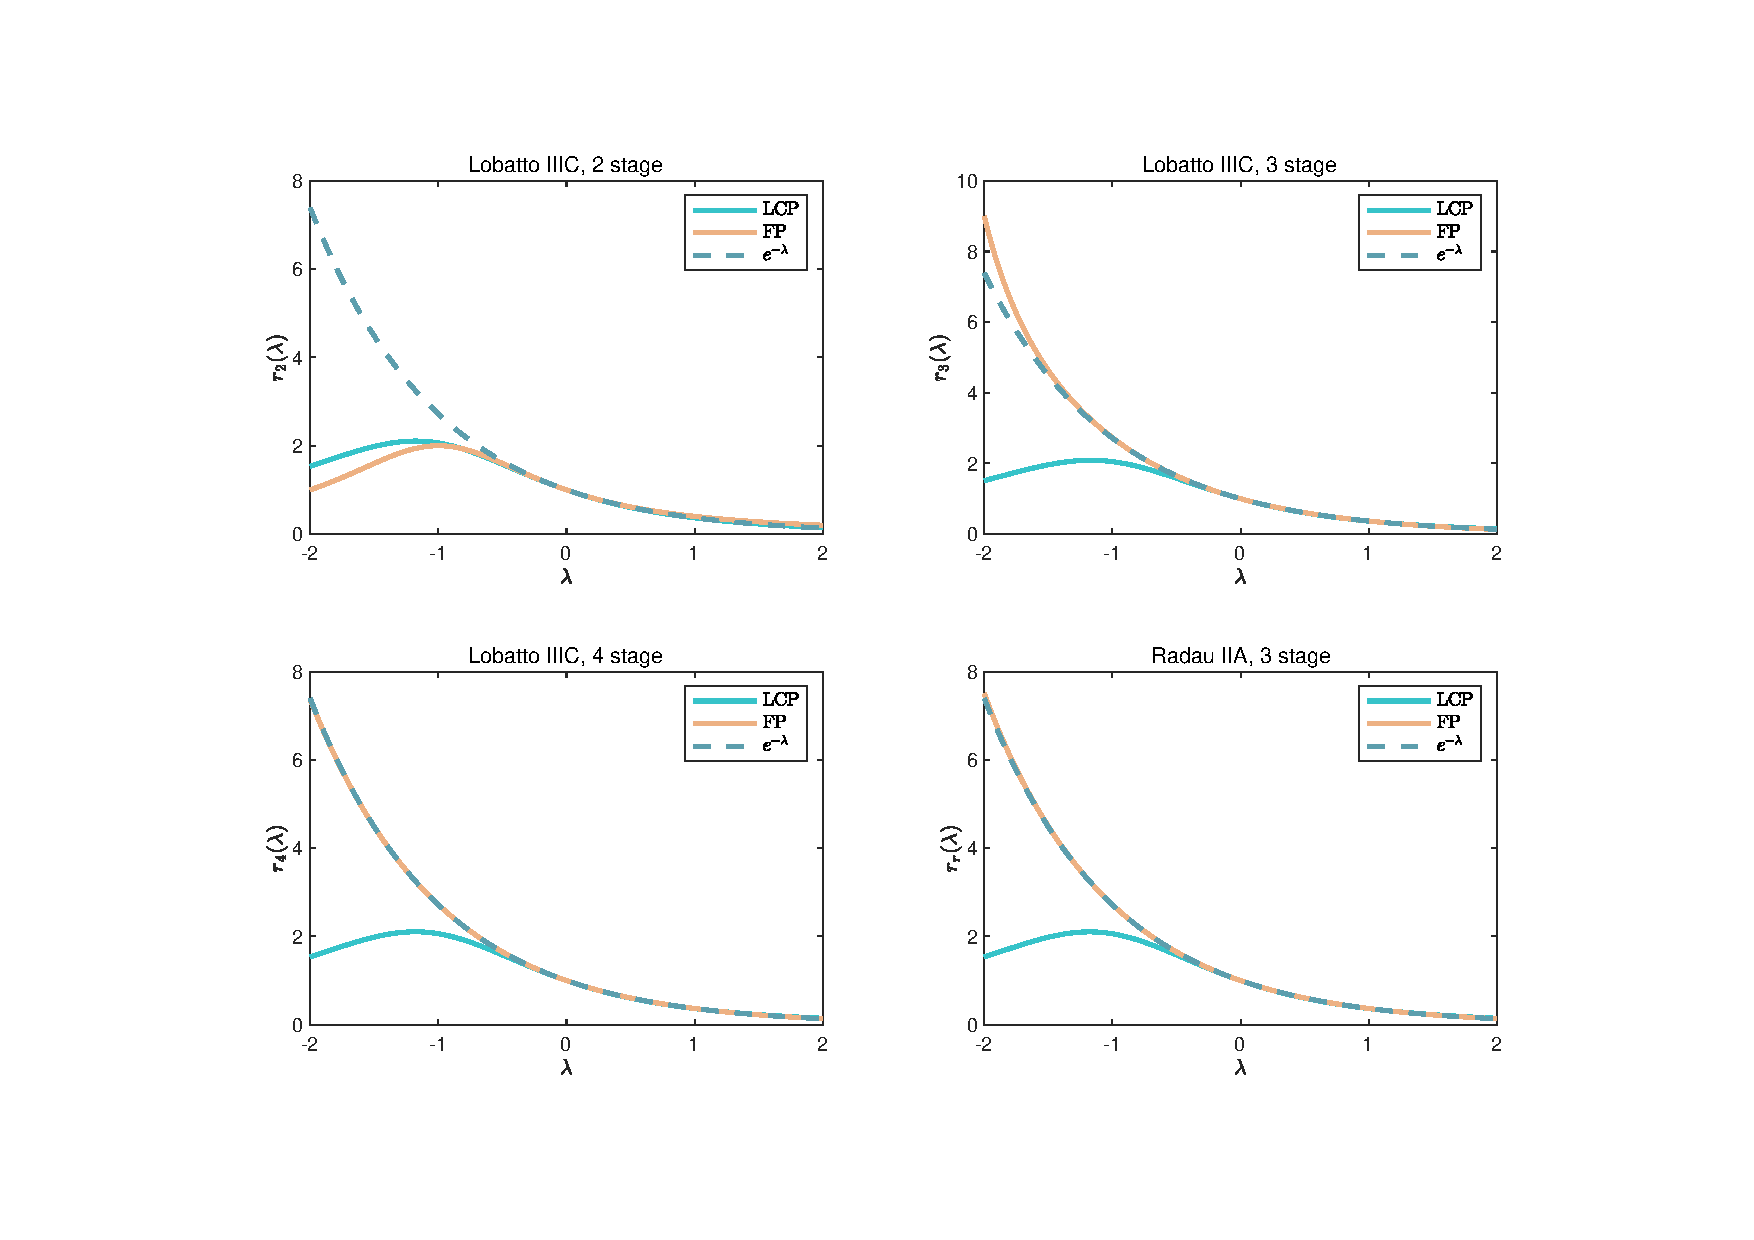
\includegraphics[width=0.8\textwidth,trim={3cm 2cm 3cm 2cm},clip]{fig_app_r.pdf}
	\caption{四种FPs的LCPs的稳定函数. }\label{fig:app_2}
\end{figure}

%% 后面可能还有《毕业论文申报表》,《指导教师评语表》等附表内容,请不要忘记
\end{document}